\documentclass[conference]{IEEEtran}
\makeatletter
\def\ps@headings{%
\def\@oddhead{\mbox{}\scriptsize\rightmark \hfil \thepage}%
\def\@evenhead{\scriptsize\thepage \hfil \leftmark\mbox{}}%
\def\@oddfoot{}%
\def\@evenfoot{}}
\makeatother
\pagestyle{headings}

\newcommand{\thetitle}{On the Linear Structure of Network Traffic: Predicting Flow Behavior}

%!TEX root = paper.tex

\usepackage[labelfont=bf,small]{caption}
\usepackage[font=small,labelfont=bf,position=top,nearskip=0em]{subfig}
\usepackage{cite,amsmath,amssymb,rotating,multirow,bigstrut,url,wrapfig,relsize,paralist,array,mathtools,units}
\usepackage[hyperfigures,bookmarks,bookmarksopen,bookmarksnumbered,colorlinks,linkcolor=black,citecolor=black,filecolor=blue,menucolor=black,pagecolor=blue,frenchlinks=true,pdftitle={\thetitle}]{hyperref}

%!TEX root = paper.tex

%% LABELING COMMANDS
\renewcommand{\sec}[1]{\label{sec:#1}}
\newcommand{\eqn}[1]{\label{eqn:#1}}
\newcommand{\fig}[1]{\label{fig:#1}}
\newcommand{\tab}[1]{\label{tab:#1}}
\newcommand{\thm}[1]{\label{thm:#1}}
\newcommand{\defn}[1]{\label{def:#1}}

%% REFERENCING COMMANDS
\newcommand{\Appendix}[1]{\hyperref[sec:#1]{Appendix~\ref*{sec:#1}}}
\newcommand{\Section}[1]{\hyperref[sec:#1]{Section~\ref*{sec:#1}}}
\newcommand{\Equation}[1]{\hyperref[eqn:#1]{Equation~\ref*{eqn:#1}}}
\newcommand{\Figure}[1]{\hyperref[fig:#1]{Figure~\ref*{fig:#1}}}
\newcommand{\Table}[1]{\hyperref[tab:#1]{Table~\ref*{tab:#1}}}
\newcommand{\Theorem}[1]{\hyperref[thm:#1]{Theorem~\ref*{thm:#1}}}
\newcommand{\Definition}[1]{\hyperref[def:#1]{Definition~\ref*{def:#1}}}

%% MATHEMATICAL NOTATIONS

% common algebraic domains
\newcommand{\N}{\mathbb{N}}
\newcommand{\Z}{\mathbb{Z}}
\newcommand{\Q}{\mathbb{Q}}
\newcommand{\R}{\mathbb{R}}

% standard operators & functors
\renewcommand{\Pr}{\mathrm{Pr}}
\newcommand{\Image}{\text{Im}}
\newcommand{\Kernel}{\text{Ker}}

% common constructs
\newcommand{\abs}[1]{{\left|#1\right|}}
\newcommand{\absx}[1]{{|#1|}}
\newcommand{\card}[1]{{\left|#1\right|}}
\newcommand{\cardx}[1]{{|#1|}}
\newcommand{\norm}[1]{{\lVert#1\rVert}}
\newcommand{\normx}[1]{{\Vert#1\Vert}}
\newcommand{\set}[1]{{\left\{#1\right\}}}
\newcommand{\setx}[1]{{\{#1\}}}
\newcommand{\parens}[1]{{\left(#1\right)}}
\newcommand{\parensx}[1]{{(#1)}}
\newcommand{\bracket}[1]{{\left[#1\right]}}
\newcommand{\bracketx}[1]{{[#1]}}
\newcommand{\seq}[1]{{\left<#1\right>}}
\newcommand{\seqx}[1]{{\lvert#1\rvert}}
\newcommand{\tuple}[1]{{\left<#1\right>}}
\newcommand{\tuplex}[1]{{\lvert#1\rvert}}
\newcommand{\floor}[1]{{\left\lfloor#1\right\rfloor}}
\newcommand{\floorx}[1]{{\lfloor#1\rfloor}}
\newcommand{\ceil}[1]{{\left\lceil#1\right\rceil}}
\newcommand{\ceilx}[1]{{\lceil#1\rceil}}
\newcommand{\round}[1]{{\left[#1\right]}}
\newcommand{\roundx}[1]{{[#1]}}
\newcommand{\fracx}[2]{{#1/#2}}
\newcommand{\fracp}[2]{{\left(\frac{#1}{#2}\right)}}
\newcommand{\fracpx}[2]{{(#1/#2)}}
\newcommand{\smallfrac}[2]{{\textstyle{\frac{#1}{#2}}}}

% standard notations
\newcommand{\trans}[1]{{#1}^T}
\newcommand{\inner}[2]{{#1}\trans{#2}}
\newcommand{\cross}{\times}
\newcommand{\tensor}{\otimes}
\newcommand{\directsum}{\oplus}
\newcommand{\iso}{\cong}
\newcommand{\union}{\cup}
\newcommand{\inter}{\cap}
\newcommand{\disunion}{\sqcup}
\newcommand{\Union}{\bigcup}
\newcommand{\Inter}{\bigcap}
\newcommand{\Disunion}{\bigsqcup}
\newcommand{\conj}{\wedge}
\newcommand{\disj}{\vee}
\newcommand{\Conj}{\bigwedge}
\newcommand{\Disj}{\bigvee}
\newcommand{\defeq}{=}
\renewcommand{\emptyset}{\varnothing}
\renewcommand{\setminus}{\,\raisebox{1pt}{$\smallsetminus$}\,}
\newcommand{\eldiv}{\,./\,}
\newcommand{\diag}{\text{diag}}
\newcommand{\rs}{\text{rs}}
\newcommand{\argmin}{\text{arg min}}

%% FORMATTING BEHAVIORS
\newcommand{\caps}[1]{{\small{#1}}}
\newcommand{\latin}[1]{\textit{#1}}
\newcommand{\defterm}[1]{\textit{#1}}
\newcommand{\newfootnote}[2]{\newcommand{#1}{\footnote{#2} }}
\renewcommand{\bullet}{\raisebox{2pt}{$\centerdot$}}
\renewcommand{\arraystretch}{1.3}

%% MISCELLANEOUS

\renewcommand{\vec}[1]{\mathbf{#1}}


\title{\vspace{-0.25em}\thetitle}
\author{
{\large{Stefan~Karpinski, John~R.~Gilbert, Elizabeth~M.~Belding}} \vspace{0.25em}\\
Department of Computer Science \\
University of California, Santa Barbara \vspace{0.35em}\\
\textit{\{sgk,gilbert,ebelding\}@cs.ucsb.edu}
}

\bibliographystyle{IEEEtran}

\newcommand{\figurename}{Figure}
\newcommand{\tablename}{Table}

\begin{document}
\maketitle

\begin{abstract}
We have observed that when network traffic behaviors are represented in vector spaces as relative frequency histograms of behavioral features, they tend to exhibit a great deal of low-rank linear structure.
We hypothesize that this structure is due the distribution of flow behaviors following a  finite mixture model.
Aside from being of theoretical interest, this hypothesis has practical consequences:
it allows us, among other things, to make detailed predictions about the probabilities of various future flow behaviors after observing only a handful of a flow's initial packets.
This practical application serves a dual function.
It provides a highly useful tool of network management, especially in wireless networks where such predictions can be leveraged to better allocate scarce bandwidth resources.
However, it also provides evidence that the hypothesized model provides a correct explanation for the observed linear structure in real network traffic.
\end{abstract}

\section{Introduction}\sec{introduction}

\newfootnote{\flownote}{We use the common definition of a \textit{flow} as a sequence of packets sharing the same  ``5-tuple'': IP protocol type, source and destination nodes, and TCP/UDP port numbers.}

This paper is the first in a three-part series employing a numerical linear algebra techniques to understand and analyze network traffic patterns at a detailed level of individual flows and packets.\flownote
All three papers employ the same analytical framework but investigate different fundamental applications of traffic modeling:
prediction, classification and generation.
In this paper we first present the framework and then demonstrate how it can predict the behavior of individual flows from the observation of only a handful of their initial packets.
% The following papers will focus on classification of flows according to application type and realistic workload generation.

This work begins with a particular way of representing flow behaviors as vectors.
% and the behaviors of entire traffic traces as large, sparse matrices.
% This approach was first proposed in by Karpinski~\emph{et~al.}~\cite{Karpinski08}, who called this general type of representation \emph{linear representations}.
The representation is quite simple.
For each feature of a flow, we represent that aspect of the flow's behavior as a \emph{feature-frequency vector}:
a vector having a dimension for each possible value of the feature and whose coordinates are the relative frequency of values.
For example, the vector representing the distribution of packet sizes of a flow having four 40-byte and two 145-bytes packets is
\begin{align}
  \text{size} = \frac{1}{6}\parens{4\vec{e}_{40} + 2\vec{e}_{145}}.
\end{align}
% The dimension of this representation is 1500 because that is typically the maximum transfer unit (\caps{MTU}) of local networks.
Different aspects of flow behavior can be represented in this way, and these representations can be combined by taking the direct sum of their representation vectors.

The behavior of any set of flows, such as a traffic trace, can be represented as a matrix of feature-frequency vectors.
We use the convection that features values correspond to matrix columns while flows correspond to matrix rows.
When traffic traces are represented like this, a very curious thing happens:
the resulting matrices exhibit a great deal of linear structure.
Specifically, flow behaviors tend to lie near the union of a small set of low-rank subspaces.
It is the investigation of this linear structure that lies at the core of this paper.

% We hypothesize that the reason for the linear structure is that the distribution of each flows behavior is a finite mixture of a small set of ``basic behaviors.''
% Moreover, the mixing of basic behaviors is itself structured.
The linear structure of network traffic allows us to perform a drastic model reduction on trace traffic patterns while preserving the essential characteristics of the original trace.
Furthermore, when observable characteristics of flows are separated from features to be predicted, this model reduction is similar to a classical linear regression:
it allows us to use least squares optimization on observed features to predict individual flow behavior.
We use this technique to predict the following characteristics of flows from a few initial packets:
\begin{enumerate}
  \item the distribution of packets sizes,
  \item the distribution of inter-packet intervals,
  \item the number of packets that will be in the flow.
\end{enumerate}
From these properties we can indirectly predict many other properties, including the total duration and data volume.

This prediction technique is clearly of immediate practical use:
applications range from network management to routing to quality of service.
Looking deeper than these applications, however, the mere fact that this prediction technique works at all provides evidence that the underlying hypothesized model of flow behavior is valid.
Our future works will provide evidence and applications by applying this model to the problems of traffic classification and realistic workload generation.

The rest of this paper is organized as follows.
In \Section{background}, we provide some background and the present the observations which motivate this work.
Our model and hypothesis about flow behavior is presented in \Section{hypothesis}.
The experimental methodology for testing this hypothesis is presented in \Section{methodology} while the results follow in \Section{results}.
\Section{discussion} discusses the meaning and impact of our results and
\Section{related-work} gives context for this work in relation prior research.
We conclude with final remarks in \Section{conclusions}.

\section{Background \& Motivation}\sec{background}\sec{motivation}

\begin{figure*}[t]
\vspace{-1em}
\begin{center}
\subfloat[\footnotesize{DARTMOUTH}]{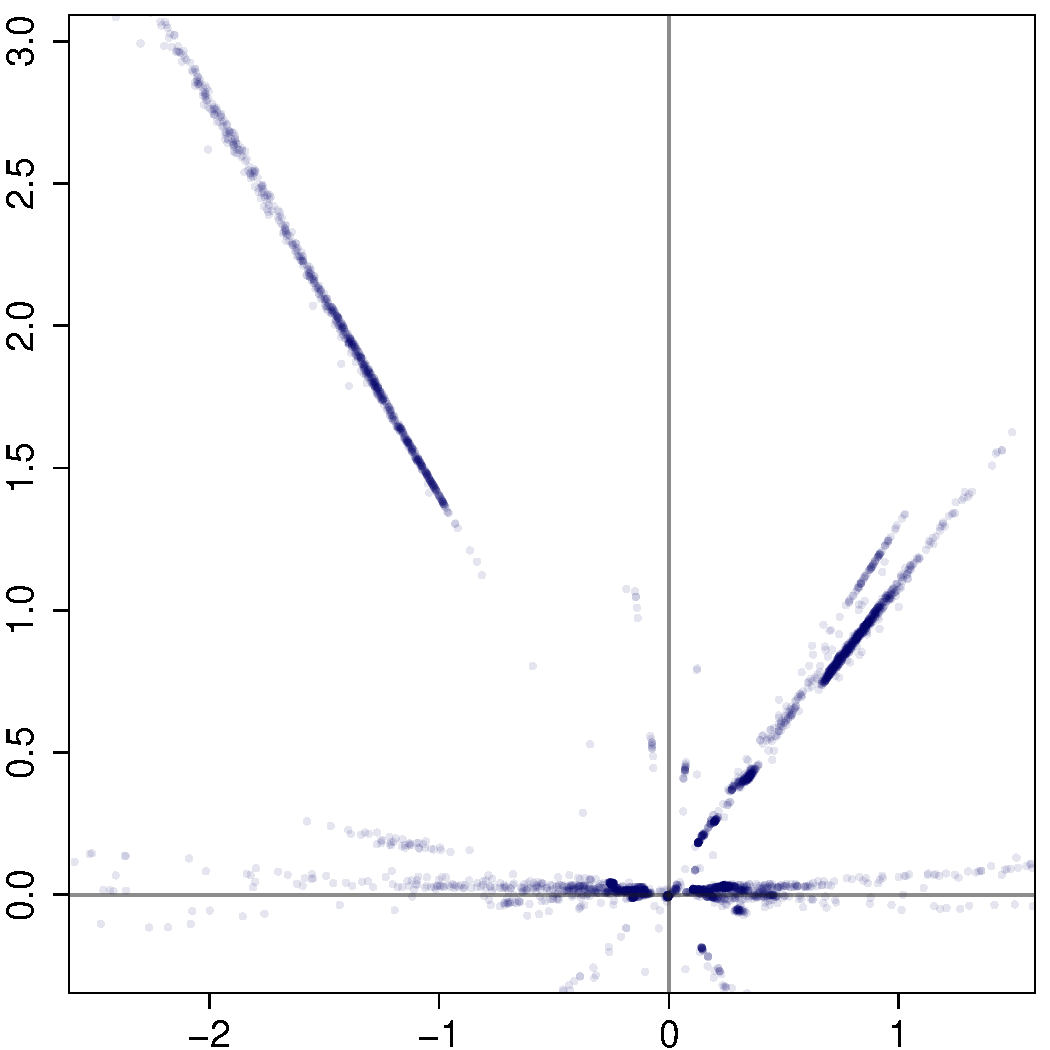
\includegraphics[width=1.15in]{svd/dart}}
\subfloat[\footnotesize{IETF 60}]{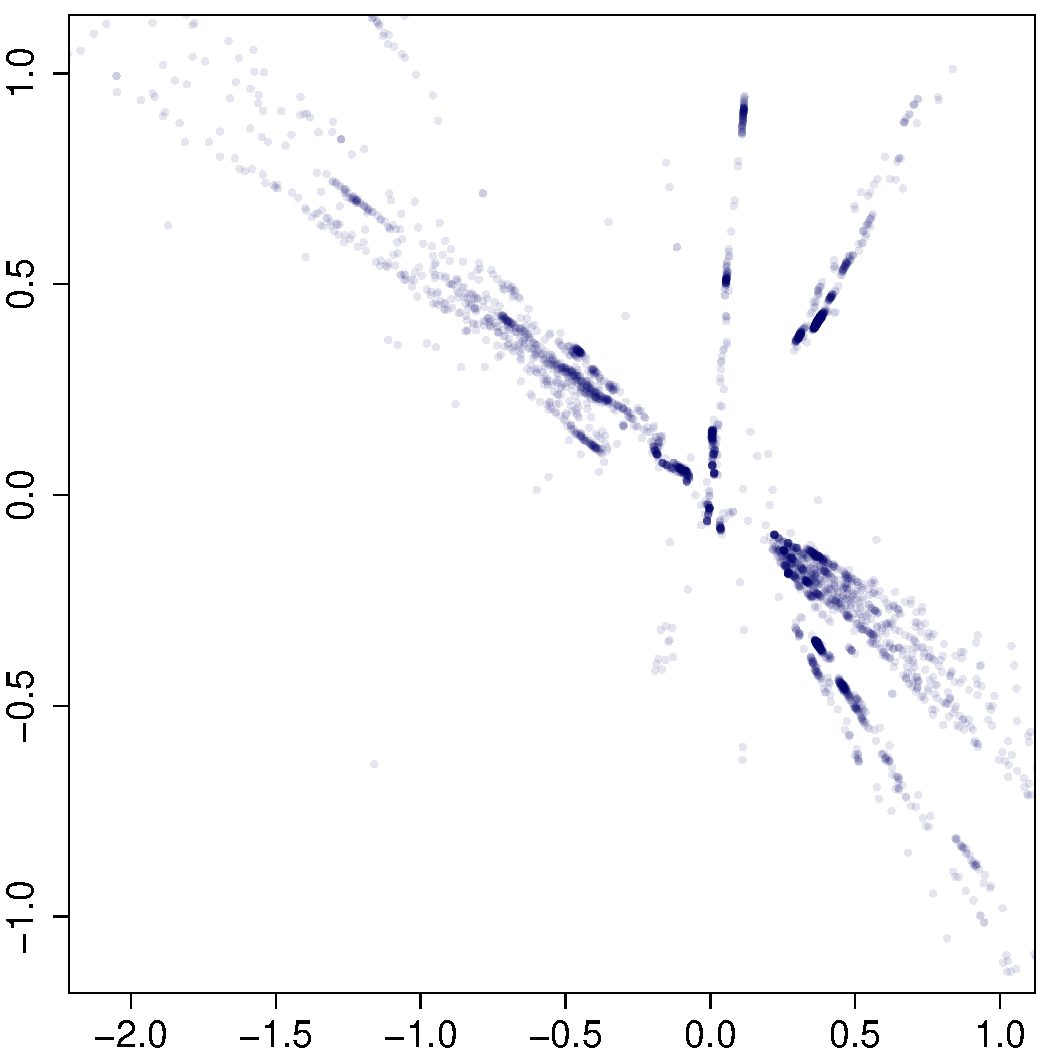
\includegraphics[width=1.15in]{svd/ie60}}
\subfloat[\footnotesize{IETF 67}]{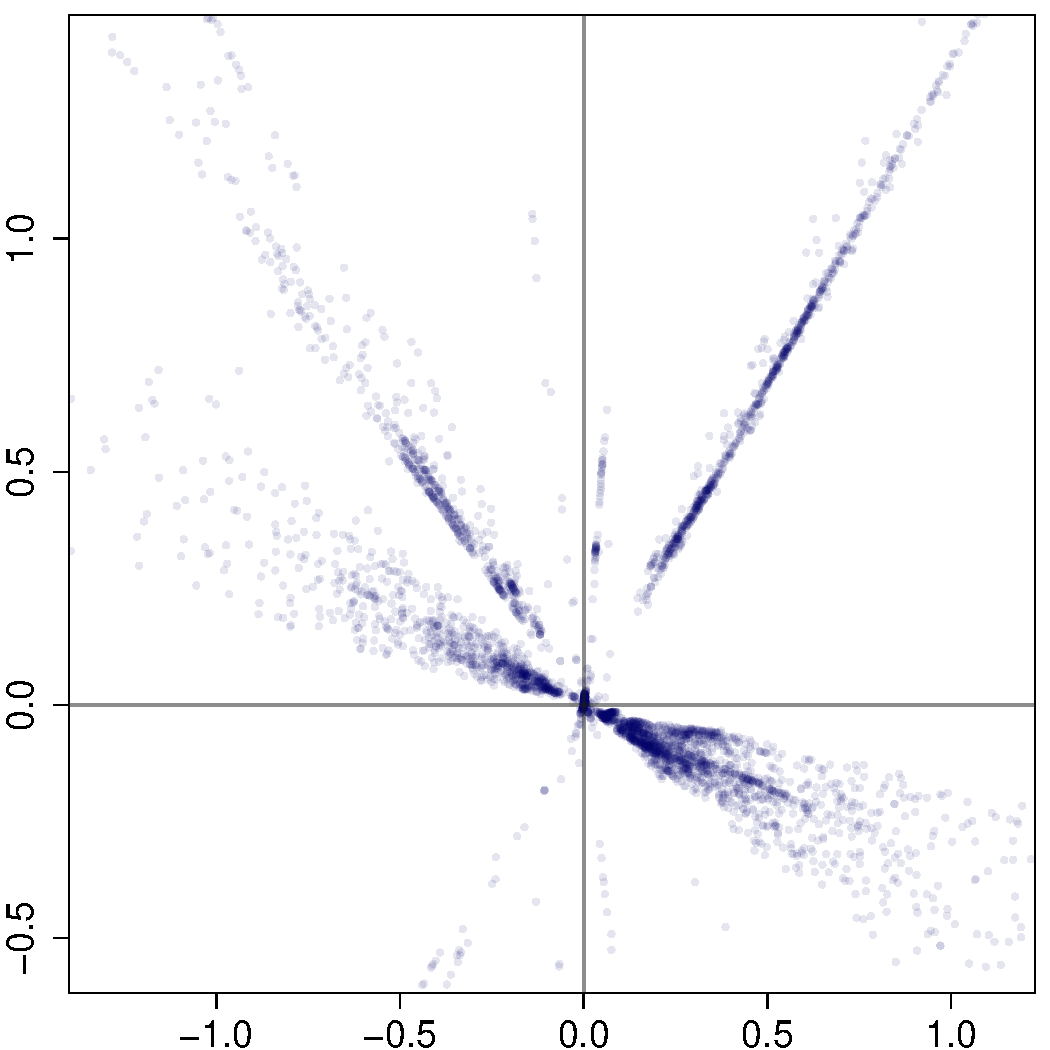
\includegraphics[width=1.15in]{svd/ie67}}
\subfloat[\footnotesize{SIGCOMM 2001}]{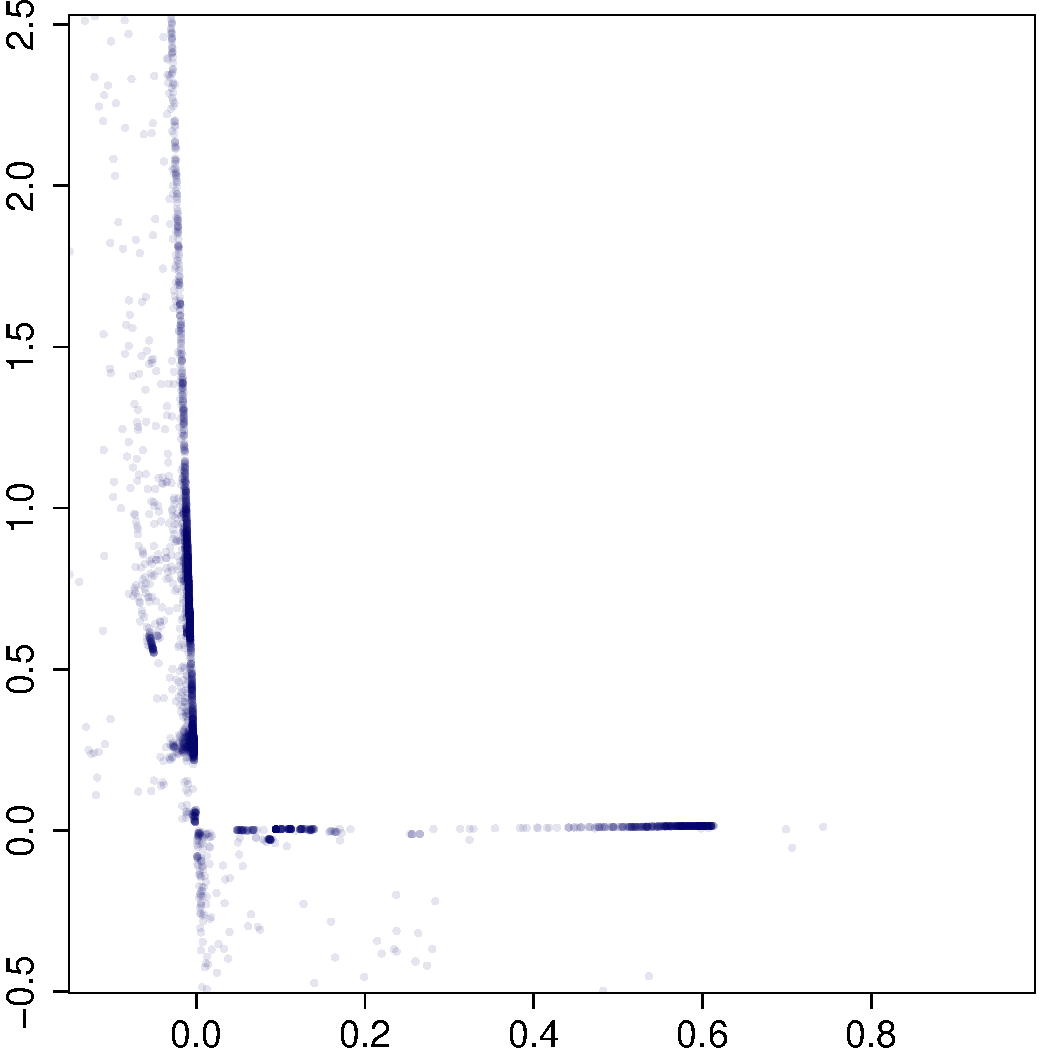
\includegraphics[width=1.15in]{svd/sc01}}
\subfloat[\footnotesize{SIGCOMM 2004}]{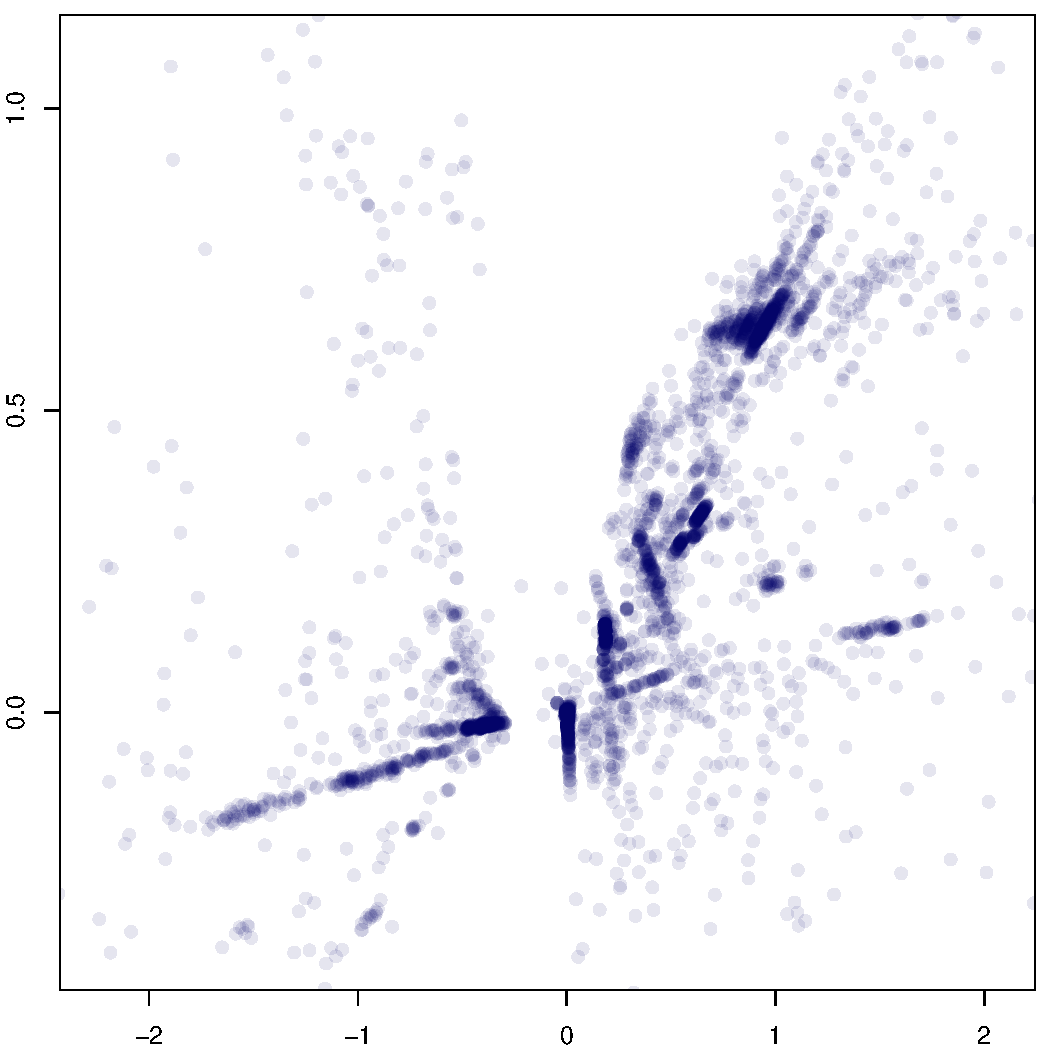
\includegraphics[width=1.15in]{svd/sc04}}
\subfloat[\footnotesize{UCSD}]{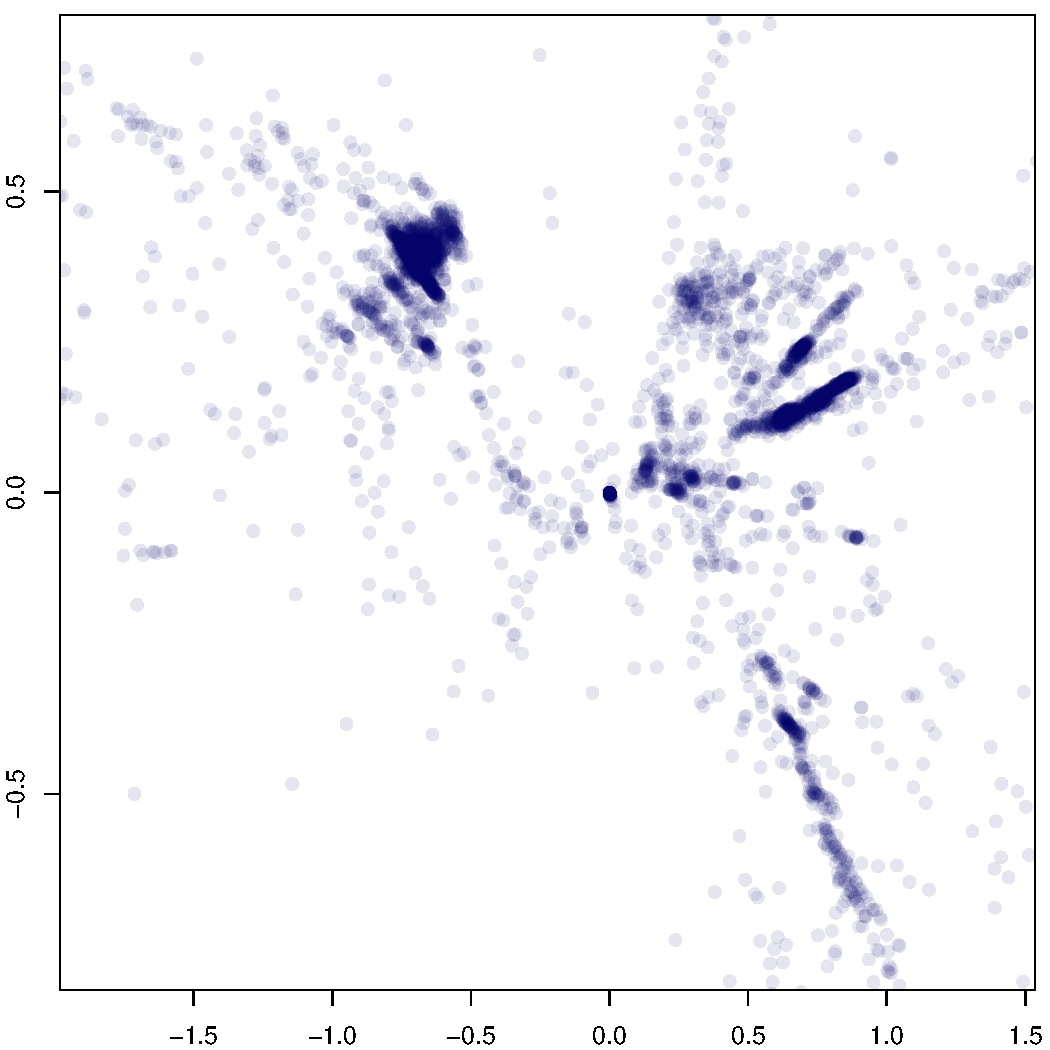
\includegraphics[width=1.15in]{svd/ucsd}}
\caption{SVD flow-behavior scatter plots for the six network traffic traces considered in this paper.} 
\fig{svd}
\end{center}
\vspace{-2em}
\end{figure*}

\newfootnote{\directsumnote}{The direct sum is the vector space analogue of a cross product of sets.}

Before we can present our motivating observation about the linear structure of network traffic, we must explain how flow behaviors are represented as feature-frequency vectors. spaces.
The low-level details of this representation are given in \Section{representation}.
For now, what the reader must know is that each feature is represented by a vector where each possible value of the feature correspond to a dimension and the normalized frequency of that value occurring is the corresponding coordinate in the vector.
We have already given the example of packet size distribution in the introduction.
The vectors are normalized in that the sum of the coordinates of each feature-frequency vector is unity.
To combine multiple feature-frequency vectors into a composite description of the overall behavior of the flow, we take the direct sum their representations:\directsumnote
\begin{align}\eqn{flow}
  \text{flow} =
  \text{size} \directsum
  \text{ival} \directsum
  \text{type} \directsum
  \text{port} \directsum
  \text{pkts}.
\end{align}
The behavior of a feature across a collection of flows can be represented as a matrix where each row represents a flow:
\begin{align}\eqn{Size}
  \text{Size} = \begin{bmatrix}
    \text{size}_1 \\
    \vdots \\
    \text{size}_m
  \end{bmatrix}.
\end{align}
The overall behavior of the collection of flows then becomes a concatenation of these feature matrices:
\begin{align}\eqn{X}
  X = \bracket{ ~
    \text{Size} ~
    \text{Ival} ~
    \text{Type} ~
    \text{Port} ~
    \text{Pkts} ~
  }.
\end{align}
It is this matrix, representing the total behavior of a collection of flows, to which we apply our analysis.

\newfootnote{\svdnote}{More precisely, the product of the first $k$ columns of $U$ with the first $k$ rows of $\trans{V}$ is a Frobenius-optimal rank-$k$ approximation of $X$.}

\newfootnote{\projectionnote}{We could normalize the vectors to unit length, but then our projection would be spherical, artificially introducing curvature into our visualization.}

To see the linear structure of these representation matrices, we apply one of the most fundamental tools of linear algebra:
the singular value decomposition (\caps{SVD}).
This matrix decomposition can be applied to any real matrix, factoring it into a product of three real matrices:
\begin{align}
  X = US\trans{V}.
\end{align}
$U$ and $V$ are orthogonal and $S$ is diagonal, with entries of nonincreasing nonnegative value.
Among the useful properties of this factorization, is that the first $k$ columns of $US$ are an optimal $k$-dimensional reduced model of $X$.\svdnote
This property allows us to visualize the structure of $X$ using initial columns of $US$---and this is precisely what we do.
However, it must be done in a particular way.
First determine an appropriate value for $k$.
Here we take the number of dimensions necessary to account for 75\% of the variance seen in $X$;
other approaches work well too.
Discarding the rest of the dimensions has the effect of ``denoising'' the data.
The vectors of the remaining $k$-dimensional reduction of $X$ may have different magnitudes, but we are only interested in direction, since vectors differing only be magnitude lie in the same one-dimensional subspace.
Therefore, we project each row vector through the origin onto the unit-sum hyperplane.\projectionnote
It is the coordinates of this reduced, projected data which exhibit clear linear structure.

\Figure{svd} shows scatter plots of most significant two coordinates when this procedure is applied to a random sample of 5000 flows from each of six independent traffic traces.
Clear linear structure is visible in all six traces:
flow behaviors are heavily concentrated near low-dimensional subspaces.
Behaviors concentrated along a one-dimensional subspace appear as dark ``spots'' where many points have been plotted;
behaviors near two-dimensional subspaces appear as lines;
behaviors on higher-dimensional subspaces appear as ``smears.''

The presence of linear structure in the matrix representations of several independent traffic traces immediately raises two significant questions.
The existential question: \emph{Why does this linear structure exist?}
Followed, of course, by the practical question: \emph{How can we exploit this structure?}
Neither question can be answered fully in a single paper, but we will begin to address the existential problem in the next section.
In the rest of this paper we apply this insight to the eminently practical problem of predicting the behavior of individual flows from the observation of only a few of their initial packets.

\section{Model \& Hypothesis}\sec{model}\sec{hypothesis}

\begin{table*}
\begin{center}
\small
\begin{tabular}{|c|c|c|c|c|c|c|}

\hline
\textbf{Trace} &
\textbf{Year} &
\textbf{Start} &
\textbf{End} &
\textbf{Type} &
\textbf{Network} \\
\hline

{\footnotesize{DARTMOUTH}} &
2003 &
Mon Nov  3 18:39:48 &
Wed Nov  5 16:09:48 &
campus &
Dartmouth College campus \\
\hline

{\footnotesize{IETF 60}} &
2004 &
Wed Aug  4 17:02:50 &
Wed Aug  4 18:02:49 &
conference &
IETF hotel venue \\
\hline

{\footnotesize{IETF 67}} &
2006 &
Wed Nov  8 19:31:56 &
Wed Nov  8 20:18:29 &
conference &
IETF hotel venue \\
\hline

{\footnotesize{SIGCOMM 2001}} &
2001 &
Wed Aug 29 17:24:47 &
Fri Aug 31 19:53:15 &
conference &
SIGCOMM hotel venue \\
\hline

{\footnotesize{SIGCOMM 2004}} &
2004 &
Tue Aug 31 13:25:04 &
Fri Sep  3 21:40:22 &
conference &
SIGCOMM hotel venue \\
\hline

{\footnotesize{UCSD}} &
2007 &
Thu Jan 11 07:59:50 &
Fri Jan 12 07:59:55 &
campus &
UCSD engineering building \\
\hline

\end{tabular}
\caption{Traffic traces used for analysis and experiments.}
\tab{traces}
\end{center}
\vspace{-2em}
\end{table*}

Our answer to the question of why low-dimensional linear structure appears in the feature-frequency representation of network traffic can be expressed as a hypothetical statistical model for flow behavior.
% A mixture model, to be specific.
We propose viewing each flow as having a probability distribution of possible behaviors it could exhibit.
% We propose that the behavior of each flow is drawn from a probability distribution on a space possible behaviors.
We hypothesize that the behavior distribution for most flows is a mixture of a relatively small set of ``basic behaviors.''
Moreover, only even smaller subsets of these basic behaviors are typically combined with each other.
Under these assumptions, we can express the distribution of each flow's behaviors as a finite mixture model~\cite{McLachlan00}:
\begin{align}\eqn{mixture-model}
  q_i(x) = \sum_{j=1}^r w_{ij} p_j(x),
\end{align}
Here $q_i$ and $p_j$ are probability density functions, and $w_{ij}$ are nonnegative weights, summing to unity for each $i$.
\Equation{mixture-model} is expressed succinctly as matrix multiplication.
Writing $Q_{ik} = q_i(k)$, $W_{ij} = w_{ij}$, and $P_{jk} = p_j(k)$, we have:
\begin{align}\eqn{mixture-model-matrix}
  Q = WP.
\end{align}
The number of basic behaviors, $r$, is the maximum possible rank of the feature distribution matrix, $Q$.
Moreover, we can partition the rows of $P$ into disjoint classes such that $w_{ij_1}$ and $w_{ij_2}$ are both non-zero only if $j_1$ and $j_2$ are in the same class.
Thus, each row of $Q$ is associated with exactly one class, and all the points associated with a class lie in the subspace spanned by its rows in $P$.

This model explains the structures found in \Figure{svd}.
Points lying along the same structure are in the same class, and each structure is ``generated'' by a small set of vertices:
the points belonging to a structure are near the convex hull generated by those vertices.
However, this is only one possible hypothesis that fits the data.
Like any hypothesis, it must be tested.
The rest of this paper, aside from providing a practical application, serves as a hypothesis test:
we try to recover the matrices $W$ and $P$ from our noisy and imperfect observations of $Q$ and use the recovered model to predict real flow behaviors.
If the recovered model can make accurate predictions, this provides evidence that our model and hypothesis are valid.

\section{Methodology}\sec{methodology}

Our experimental procedure has three parts:
training, prediction and evaluation.
For training, we take a sample of network trace traffic and attempt to recover the model hypothesized in \Section{hypothesis} from it.
We use the trained model to predict behaviors of a separate set of flows from the same trace, using only knowledge of a few initial packets of each flow.
Finally, we must evaluate the quality of these predictions by comparing them to the actual behavior of those flows.
In this section we present the methodology for training and prediction;
how to evaluate prediction results against actual behavior is left until the next section together with the results.

% It seems wise at this point to address the nature of prediction for highly nondeterministic phenomena like network traffic.
% Brief reflection shows that one cannot hope to accurately predict the exact behavior of flows:
% flows may exhibit the same initial behavior but subsequently behave quite differently.
% The best we can do then is to predict a \emph{distribution} of possible outcomes given the observed initial behavior.
% When compared with a specific outcome, such a prediction cannot be said to be ``wrong'' or ``right.''
% How then can one measure the quality of a predicted distribution of outcomes?
% This subtle and difficult issue is central to our evaluation methodology.

\subsection{Data Sets}

We use randomly sampled traffic from six different network traces.
All six traces are freely available from the \caps{CRAWDAD} wireless trace repository~\cite{Yeo06}.
Details of the traces are shown in \Table{traces}.
These traces represent a broad cross-section of traffic patterns over time and a reasonable variety of network types.
Unfortunately, we could not find any freely available residential or corporate network traces that were usable for our analysis.
We randomly sampled 5000 flows from each trace for training and another 5000 flows for testing.

\subsection{Feature-Frequency Representation}\sec{representation}

We embed the following features of flow behavior into vector spaces via feature-frequency representation:
packet size distribution,
inter-packet interval distribution,
\caps{IP} protocol type,
\caps{TCP/UDP} port numbers,
and packet count.
Packet sizes are already naturally discrete, taking on only values from 1 to the \caps{MTU}, which was 1500 in all of our traces.
Inter-packet intervals must be quantized, using the scheme described by Karpinski~\emph{et~al.}~\cite{Karpinski08} but using only 500 dimensions instead of 1500.
This scheme maps bins of interval durations to indices, with the bins starting at the scale of milliseconds, but ramping smoothly up to seconds at the high end of the scale.
Intervals of more than ten minutes are considered to start a new flow.
\caps{IP} protocol type also naturally discrete, with values from 0 to 255, represented by a 256-dimensions histogram vector.
The feature-frequency vector for a single flow in this case is always just a vector with a single unit entry and all other entries zero.
Port numbers are naturally discrete as well, but the range of port numbers (0-65535) is too large for practical representation using a full histogram.
Instead, we represent port numbers by their remainder modulo 1000.
Port numbers are sufficiently spread out that this still provides ample distinction between traffic types.
Moreover, since the direction of a flow is generally uninteresting, we represent both source and destination in a single vector containing two values.
We also represent the packet count of each flow.
Since the potential packet count is unlimited, some approach is needed for limiting the dimension of this frequency representation.
We use the simplest approach and simply cap the packet count at 3000 packets:
all flows with 3000 or more packets fall into the same histogram bin and are simply considered ``very large.''

\subsection{Model Recovery}\sec{model-recovery}

\subsubsection{Subspace Segmentation}\sec{subspace-segmentation}

Once the data have been expressed in matrix form, the next step is attempt to detect the linear structures seen in \Figure{svd}.
% Recall that these correspond to the point classes in our hypothesized model.
We use Ma~\emph{et~al.}'s~\cite{Ma07} algorithm for segmenting multivariate data into a union of subspaces using lossy data coding and compression.
The essential idea of this algorithm is to compute the number of bits needed to encode the data under various assumed groupings.
The grouping which yields the best compression is the desired segmentation.
This algorithm has many desirable qualities.
Two are essential:
1) unlike most clustering algorithms, it finds subspaces, not regions;
2) it is highly robust to outliers and noisy data.
The algorithm has one parameter:
the maximum allowable distortion of the data
We follow Ma's lead when applying the algorithm to \caps{SVD} data and use $\varepsilon^2 = 1$.
The result of this stage is a segmentation of the data into classes of rows, precisely as our hypothesized model requires.

\subsubsection{Subspace Factorization}\sec{subspace-factorization}

\newfootnote{\svdnnnote}{The first singular vector of a nonnegative matrix is guaranteed to be nonnegative, but the other singular vectors will have mixed sign.}

The next step towards recovering the structure of the hypothesized model is to determine the hull points of each linear substructure.
We have determined, as well as we can, which $q_i$ belong to the same structures.
Now we must determine the vertices, $p_j$, which generate these structures.
We can use \caps{SVD} to determine the most prominent linear components of each structure, but \caps{SVD} will give us vectors of mixed sign.\svdnnnote
Since negative probability distributions are meaningless, these do not give us a plausible recovery of our model.
We must turn to other techniques to recover possible vectors for the $p_j$.

In essence, what we have is a nonnegative matrix factorization (\caps{NMF}) problem:
if $Q_*$ is a sub-matrix of rows in the same structure class, we want to find nonnegative matrices, $W_*$ and $P_*$, such that $Q_* \approx W_* P_*$.~
% We have the additional constraint that $W_*$ and $P_*$ have unit-sum rows, but that can easily be guaranteed since 
$P$ is a vertical concatenation of the $P_*$ matrices, while $W$ is a direct sum of $W_*$ matrices.
Many \caps{NMF} algorithms have been proposed since Lee and Seung published the first~\cite{Lee01}.
We use Kim and Park's alternating non-negative least squares (\caps{ANLS}) algorithm~\cite{Kim08:anls} first for its rapid initial convergence, but refine the result using Lee and Seung's Euclidean algorithm.

\newfootnote{\cddnote}{To do this, we use Avis and Fukuda's vertex enumeration algorithm as implemented in Fukuda's excellent CDD library~\cite{Avis92}.}

We find that using the standard random \caps{NMF} initialization does not yield factorizations of sufficient quality, so we have developed the following initialization procedure.
Reduce the data to the number structural dimensions sought using \caps{SVD}.
Cluster the reduced data points into one cluster per structural dimension using $k$-means clustering.
Use cluster membership from this step to combine the original data, leaving only one composite row per desired structural dimension.
These rows provide a ``denoised'' set of nonnegative spanning vectors that estimate the true low-dimensional subspace from which the data were sampled.
Finally, we find the intersection of this subspace with the standard simplex in $\R^n$.\,\cddnote
This step gives us a set of nonnegative vertices geometrically guaranteed to contain all of the estimated low-dimensional subspace.
These vectors are used to initialize the \caps{NMF} algorithms, yielding extremely good factorization for small substructures.

\subsection{Flow Behavior Prediction}\sec{flow-behavior-prediction}

In order to perform flow behavior prediction, we separate the flow features into the observable ones and the ones that must be predicted.
For example, if we want to predict total flow behavior from some number of initial packets, then we would have the following matrix of observables:
\begin{align}
  X_\text{o} = \bracket{ ~
    \text{Size}_{\text{init}} ~
    \text{Ival}_{\text{init}} ~
    \text{Type} ~
    \text{Port} ~
  }
\end{align}
The matrix of ``predictables'' would be:
\begin{align}
  X_\text{p} = \bracket{ ~
    \text{Size}_{\text{rest}} ~
    \text{Ival}_{\text{rest}} ~
    \text{Pkts} ~
  }
\end{align}
We use the packet sizes and inter-packet intervals of the initial packets, together with their \caps{IP} type and port numbers to predict the distribution of packets sizes and inter-packet intervals for the rest of the flow, as well as predicting a distribution of possible of packet counts.
In order to do this prediction, subspace factorization must be done with the observable and predictable matrices separated.
That is, subspace factorization must be done on the matrix $[X_\text{o}~X_\text{p}]$.
% However, we perform our subspace segmentation step on the combined data as in \Equation{X}.
% Why the difference? We have two pragmatic reasons:
% 1) the segmentation step seems to work better with the unseparated matrix.
% 2) we want to apply our prediction technique with different numbers of initial packets;
% the segmentation step is very slow, while the factorization step is relatively fast;
% this way we can use the same segmentation result for varying numbers of initial packets.

Our technique is fundamentally similar to fitting a regression line to noisy two-dimensional training data and then using the $x$-coordinates of test data points to linearly predict the $y$-coordinates.
The main differences are the vastly higher number of dimensions and more complex structure we assume for our data.
From the training data, we recover our estimated version of the $P$ matrix.
We split this into its observable and predictable parts: $P_\text{o}$ and $P_\text{p}$.
Given an observation matrix, $X^*_\text{o}$, to perform prediction, we find the nonnegative matrix of weights, $W_*$, minimizing the squared Frobenius error:
\begin{align}
  \norm{X^*_\text{o} - W^* P_\text{o}}^2_\text{frob}.
\end{align}
This is equivalent to minimizing the square error for each observation individually, but optimizing \emph{en masse} allows fast non-negative least squares algorithms to be used~\cite{Benthem04,Kim08:block-pivot}.
The predicted behavior for these flows is simply the weight matrix times the predictable feature matrix:
\begin{align}
  X^*_\text{p} = W^* P_\text{p}.
\end{align}
The rows of $X^*_\text{p}$ are our predictions about the behavior of flows observed in $X^*_\text{o}$.
Each row contains a packet size distribution, an inter-packet interval distribution and a distribution of packet counts.

% With our hypothetical model parameters, $p_j$, extracted from training data, for each test observation, $q^*_\text{o}$, we find nonnegative weights, $w^*_j$, that minimize the squared error
% \begin{align}\textstyle
%   \norm{q^*_\text{o}-\sum {w^*_j p_j}}^2.
% \end{align}
% The predicted behavior of the flow is simply 

\section{Results}\sec{results}

\begin{figure*}[t]
\vspace{-1em}
\begin{center}
\subfloat[Packet sizes: \footnotesize{DARTMOUTH}]{%
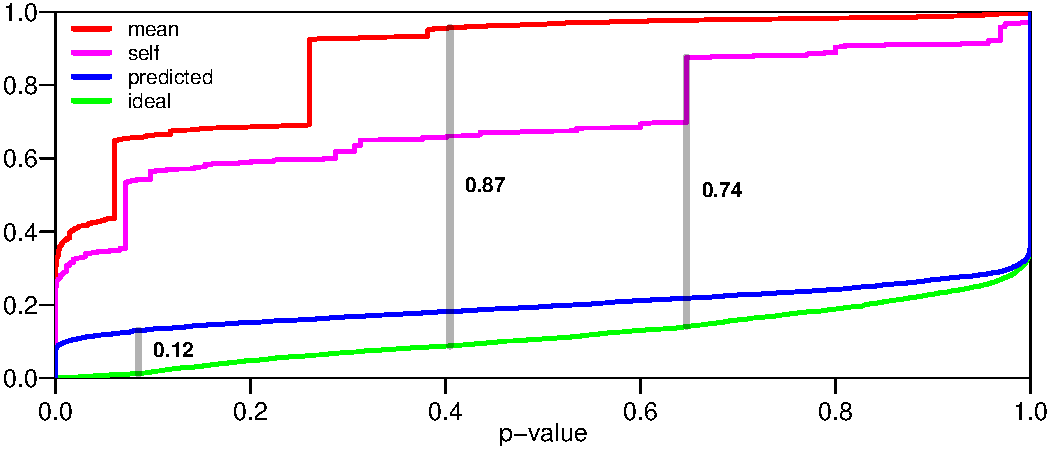
\includegraphics[width=3.545in]{size/dart}}
\subfloat[Packet sizes: \footnotesize{SIGCOMM 2004}]{%
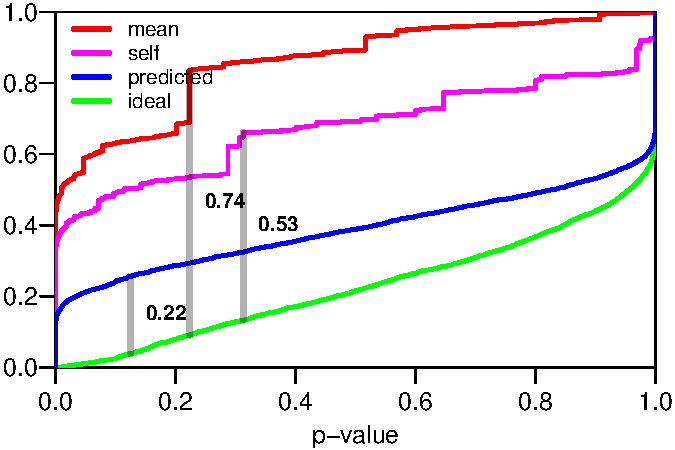
\includegraphics[width=3.545in]{size/sc04}}
\subfloat[Inter-packet intervals: \footnotesize{DARTMOUTH}]{%
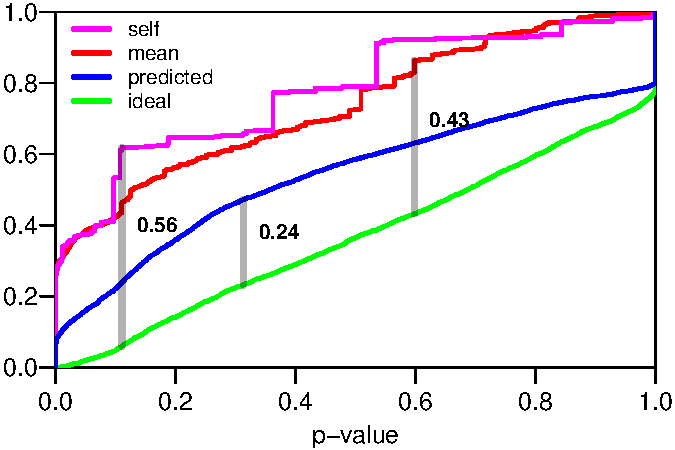
\includegraphics[width=3.545in]{ival/dart}}
\subfloat[Inter-packet intervals: \footnotesize{SIGCOMM 2004}]{%
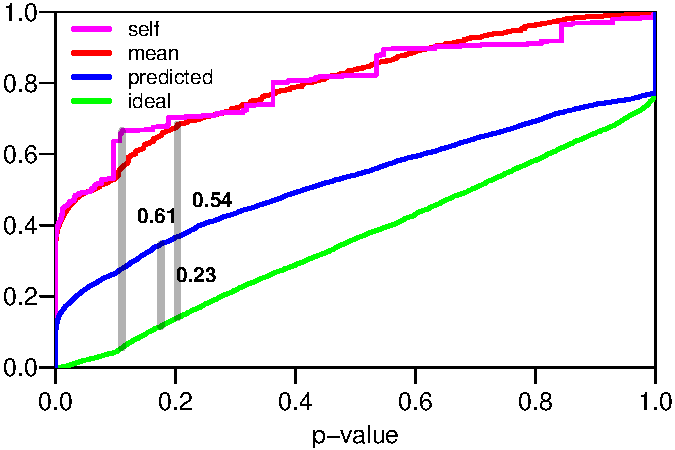
\includegraphics[width=3.545in]{ival/sc04}}
\caption{%
Empirical CDFs of Kolmogorov-Smirnov p-values for various predictors of packet size distribution and inter-packet interval distribution for two selected traces. Lower curves are better and the ideal curve provides a lower bound on quality.
Vertical segments indicate the farthest distance between the ideal and each CDF.
This distance serves as a pessimistic measure of each predictor's error rate.
}
\fig{cdf}
\end{center}
\vspace{-1em}
\end{figure*}

\begin{figure*}[t]
\begin{center}
\hfill
\subfloat[Packet count: accuracy]{%
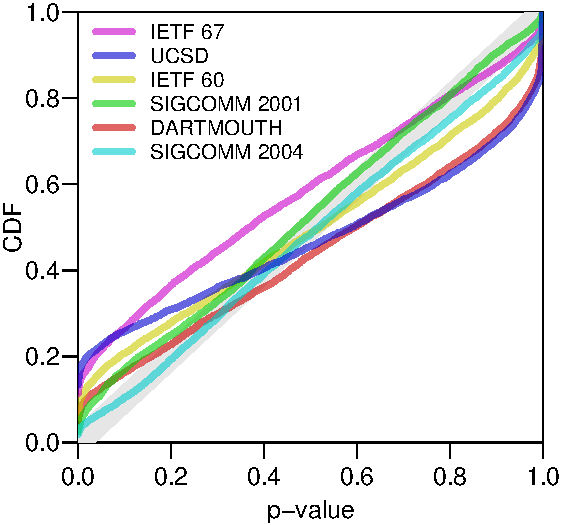
\includegraphics[width=2.1in]{pkts_accuracy}}\hfill
\subfloat[Packet count: uncertainty reduction]{%
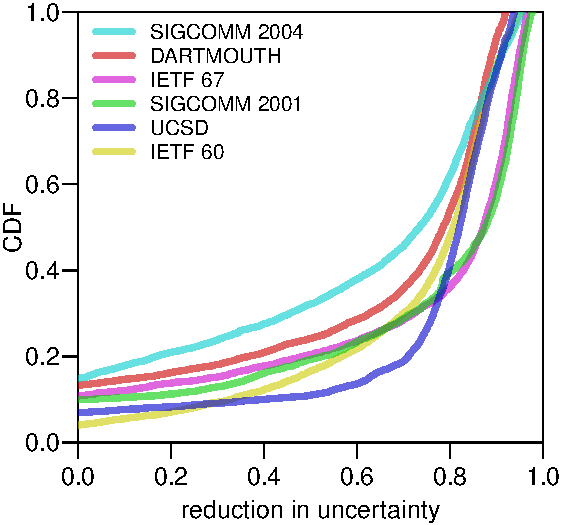
\includegraphics[width=2.1in]{pkts_certainty}}\hfill
\subfloat[Packet count: prediction entropy]{%
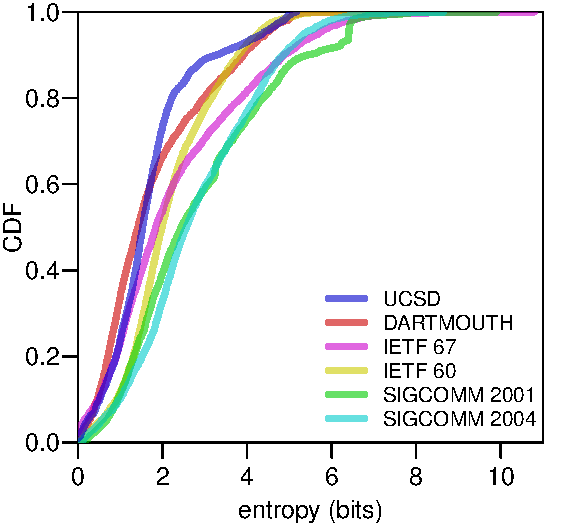
\includegraphics[width=2.1in]{pkts_entropy}}\hfill
\caption{Packet count prediction accuracy, uncertainty reduction and entropy.}
\fig{packets-accuracy}
\end{center}
\vspace{-2em}
\end{figure*}

\section{Discussion}\sec{discussion}

\section{Related Work}\sec{related-work}

\section{Conclusions}\sec{conclusions}

\bibliography{IEEE,references}

\end{document}
